\documentclass{beamer}
\usepackage[T1]{polski}
\usepackage[polish]{babel}
\usepackage[utf8]{inputenc}
\usepackage[T1]{fontenc}
\usepackage[mediumspace,mediumqspace,Grey,squaren]{SIunits}
\usepackage{graphicx}
\usepackage{filecontents}

%\addbibresource{bibliography.bib}

%\setbeamertemplate{bibliography item}{\insertbiblabel}


\graphicspath{ {images/} }

\begin{document}
\title{Ryż mydło i powidło}   
\author{Jakub Arnold Postępski} 
\date{\today} 

\frame{\titlepage} 


\section{Wstęp}

\frame{

	\frametitle{Systemy czasu rzeczywistego}
	Urządzenie techniczne, którego wynik i efekt działania jest zależny od chwili wypracowania tego wyniku. \cite{wiki:RTC}\\
	\vspace{1in}
	Systemy dzielimy na:
	\begin{itemize}
		\item Twarde
		\item Sztywne
		\item Miękkie
	\end{itemize}
}
	
\frame{
	\frametitle{Budowa ogólna}
	Budowę można obrazować standardowym modelem ISO/OSI. W praktycznych realizacjach część z warstw jest pomijana
	\begin{itemize}
		\item Fizyczne urządzenia i magistrale
		\item Algorytmy transportu danych
		\item Sterownik systemu operacyjnego
		\item Aplikacja
	\end{itemize}
}



\frame{
	\frametitle{Co chcemy uzyskać? - Sieci telekomunikacyjne}
	\begin{itemize}
		\item Telekomunikacja
		\item Kontrola systemów infrastruktury
		\item Automotive
		\item Medycyna
		\item Wojskowość
		\item Petrochemia
		\item Energetyka
		\item Robotyka
	\end{itemize}
}

\frame{
	\frametitle{Co chcemy łączyć? - Urządzenia}
		\begin{figure}
			\centering
			\includegraphics[width=0.99\linewidth,page=2]{motherboard}
			\caption{Schemat ideowy płyty głównej laptopa \cite{image:motherboard}}
			\label{fig:motherboard}
		\end{figure}
	}

\frame{\frametitle{Przykłady urządzeń}
	\begin{itemize}
		\item Linux z patchem RT
		\item BeagleBone
		\item $\micro$C na przerwaniach
		\item $\micro$C z pseudo systemem operacyjnym
		\item PLC
		\item FPGA
	\end{itemize}
	}
\frame{
	\frametitle{Rodzaje łącz}
	\begin{itemize}
		\item Przewodowe
		\item Bezprzewodowe
		\item Światłowodowe
	\end{itemize}
	\begin{itemize}
		\item Analogowe
		\item Cyfrowe
		\item Ze zwielokrotnieniem falowym
	\end{itemize}
	\begin{itemize}
		\item Szeregowe
		\item Równoległe
	\end{itemize}
}

\frame{
	\frametitle{Otwarty kolektor/dren}
	\begin{figure}
		\centering
		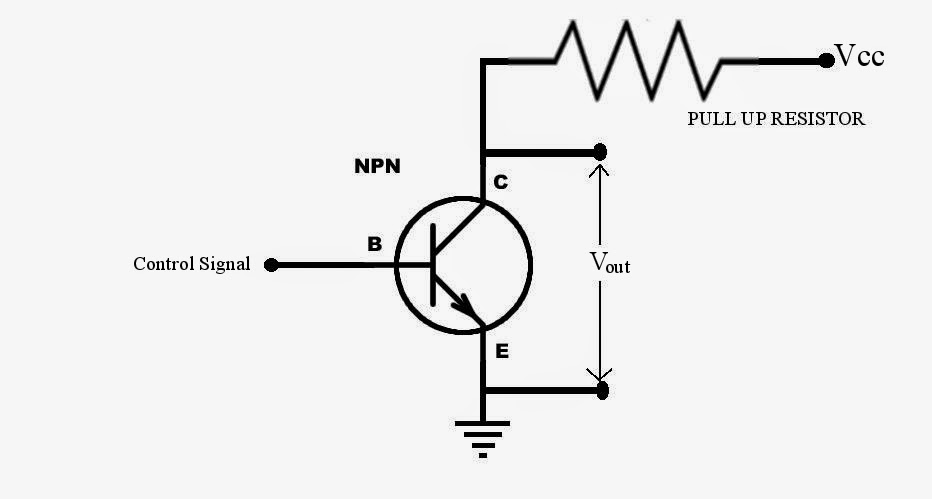
\includegraphics[width=0.9\linewidth]{open_collector}
		\caption{Schemat otwartego kolekotra\cite{image:collector}}
		\label{fig:open_collector}
	\end{figure}
}

\frame{
	\frametitle{Optoizolacja}
	
	}

\frame{
	\frametitle{Para różnicowa}
	\begin{figure}
		\centering
		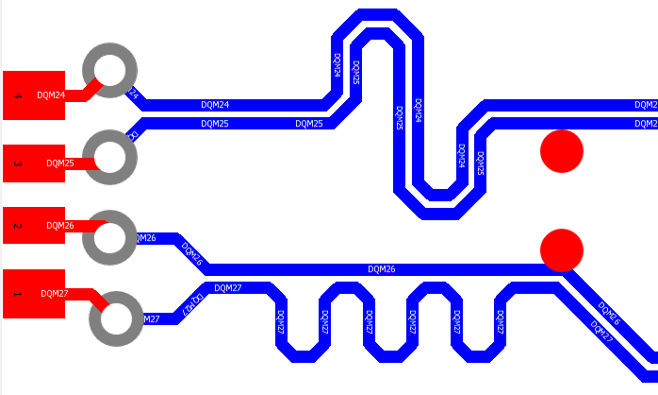
\includegraphics[width=0.9\linewidth]{differential}
		\caption{Przykładowa realizacja pary różnicowej na PCB\cite{image:collector}}
		\label{fig:differential}
	\end{figure}
}

\frame{
	\frametitle{Wzmacniacz operacyjny}
	\begin{figure}
		\centering
		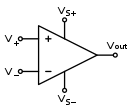
\includegraphics[width=0.9\linewidth]{wzmacniacz}
		\caption{Symbol wzmacniacza operacyjnego
			\cite{image:wzmacniacz}}
		\label{fig:wzmacniacz}
	\end{figure}
}

\frame{
	\frametitle{Budowa światłowodu}
	\begin{figure}
		\centering
		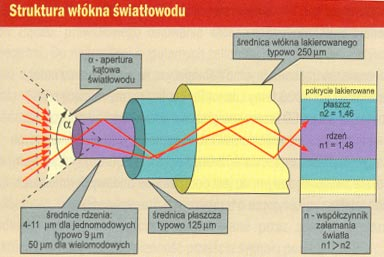
\includegraphics[width=0.9\linewidth]{swiatlowod3}
		\caption{Budowa światłowodu
		\cite{image:swiatlowod}}
		\label{fig:swiatlowod1}
	\end{figure}
}

\frame{
	\frametitle{Rodzaje światłowodów}
		\begin{itemize}
			\item Wielomodowe
			\item Jednomodowe
		\end{itemize}
		
		\begin{itemize}
			\item Skokowe
			\item Gradientowe
		\end{itemize}
		
		\begin{itemize}
			\item Plastikowe
			\item Szklane (np. SiO$_2$)
			\item Półprzewodnikowe (np. GaAs)
		\end{itemize}
	}
	
\frame{
	\begin{figure}
		\centering
		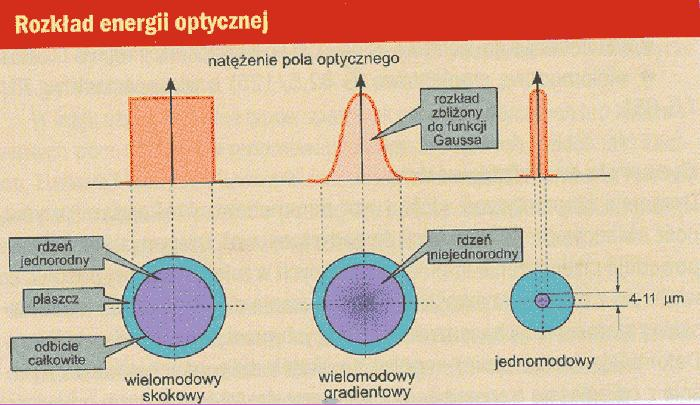
\includegraphics[width=0.9\linewidth]{swiatlowod1}
		\caption{Wyjście światłowodu
			\cite{image:swiatlowod}}
		\label{fig:swiatlowod3}
	\end{figure}
}

\frame{
	\frametitle{Łączenie światłowodu}
	\begin{itemize}
		\item Trwałe
		\item Rozłączne
	\end{itemize}
	
	\begin{figure}
		\centering
		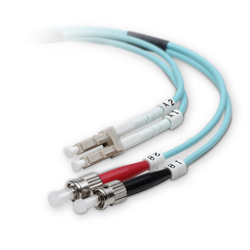
\includegraphics[width=0.5\linewidth]{swiatlowod4}
		\caption{Złącze LC i ST (dół)
			\cite{image:zlacze}}
		\label{fig:swiatlowod4}
	\end{figure}
	
}


\frame{
	\frametitle{Światłowody}
	
	
	\begin{itemize}
		\item Prędkości nawet rzędu Tb/s
		\item Małe tłumienie - duże odległości
		\item Brak problemów elektromagnetycznych (także bezpieczeństwo)
		\item Problemy z fizycznymi połączeniami
		\item Wrażliwość na uszkodzenia
		\item Koszt wykonania
	\end{itemize}
	
	Lasery klasy pierwszej są bezpieczne. Lasery klasy czwartej mogą powodować choroby oczu, oparzenia i pożar.
}




\frame{
	\frametitle{Przepustowość}
	In computing, bandwidth is the bit-rate of available or consumed information capacity expressed typically in metric multiples of bits per second. Variously, bandwidth may be characterized as network bandwidth, data bandwidth, or digital bandwidth. \cite{wiki:Przepustowosc}
	\\Zależy od jakości ośrodka, w tym:
	\begin{itemize}
		\item Fizycznej realizacji
		\item Algorytmów kompresji
		\item Algorytmów korekcji błędów
		\item (Ilości węzłów w sieci)
	\end{itemize}
}




\frame{
	\frametitle{Problemy z nadawaniem}
	\begin{itemize}
		\item Half duplex
		\item Full duplex
	\end{itemize}
	
	\begin{itemize}
		\item Jeden master
		\item Wiele masterów
		\item Wykrywanie kolizji
		\item Tokeny
	\end{itemize}
}




\frame{
	\frametitle{Transport danych}
	\begin{itemize}
		\item Enkapsulacja
		\item Kompresja
		\item Korekcja błędów
		\item Obsługa kolizji
	\end{itemize}
}


\frame{
	\frametitle{RS-232}
	\begin{itemize}
		\item 2 urządzenia
		\item 15 m
		\item Wybrane prędkości: 50, 9600, 115200, 921600 bit/s 
	\end{itemize}	
}

\frame{
	\frametitle{RS-232}
		\begin{figure}
			\centering
			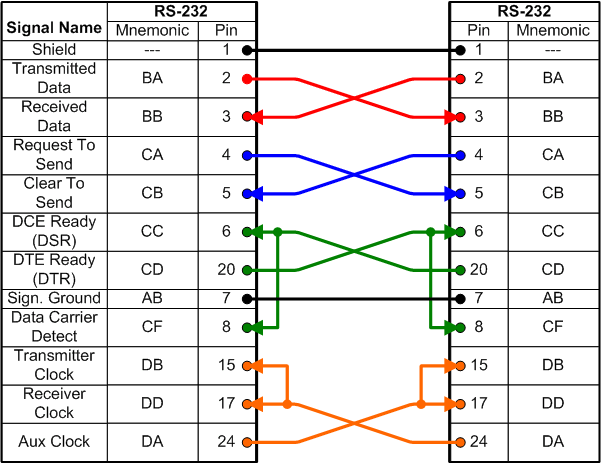
\includegraphics[width=0.9\linewidth]{rs232pin}
			\caption{Piny standardu RS232
				\cite{image:rs232pin}}
			\label{fig:rs232pin}
		\end{figure}
	}

\frame{
	\frametitle{RS-232}
	\begin{figure}
		\centering
		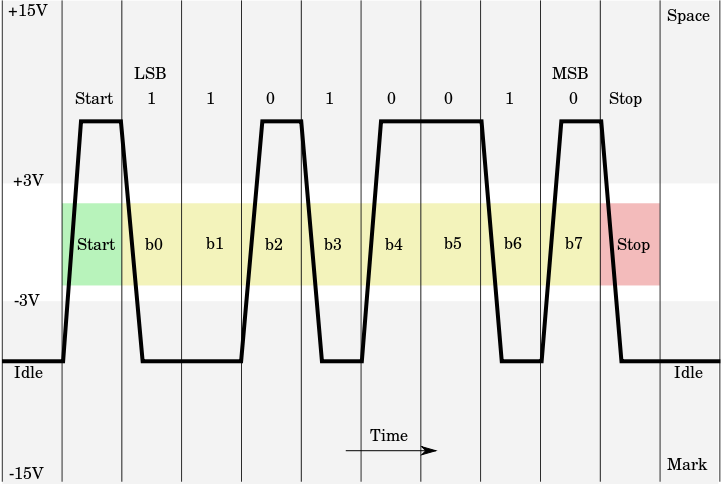
\includegraphics[width=0.9\linewidth]{rs232}
		\caption{Listing przesłania ramki
			\cite{image:rs232}}
		\label{fig:rs232}
	\end{figure}
}


\frame{
	\frametitle{RS-485}
	\begin{itemize}
		\item 32 urządzeń
		\item 1200 m
		\item 10 Mbit/s
		\item Sygnał różnicowy
		\item Half-duplex
	\end{itemize}
	\begin{figure}
		\centering
		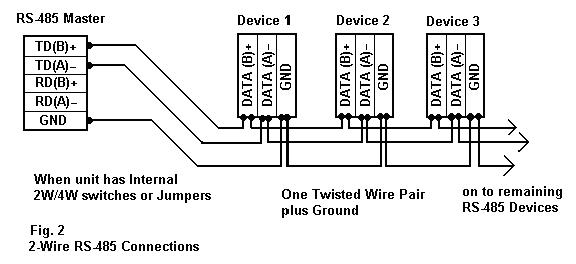
\includegraphics[width=0.7\linewidth]{rs485polaczenie}
		\caption{Schemat połączenia urządzeń
			\cite{image:rs485polaczenie}}
		\label{fig:rs485polaczenie}
	\end{figure}	
}

\frame{
	\frametitle{RS-485 vs RS-232}
	\begin{figure}
		\centering
		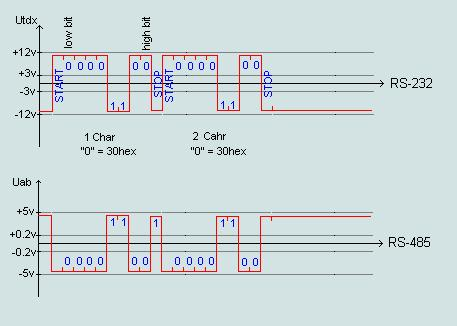
\includegraphics[width=0.9\linewidth]{rs485ramka}
		\caption{Schemat połączenia urządzeń
			\cite{image:rs485ramka}}
		\label{fig:rs485ramka}
	\end{figure}	
}

\frame{
	\frametitle{Modbus}
	\begin{figure}
		\centering
		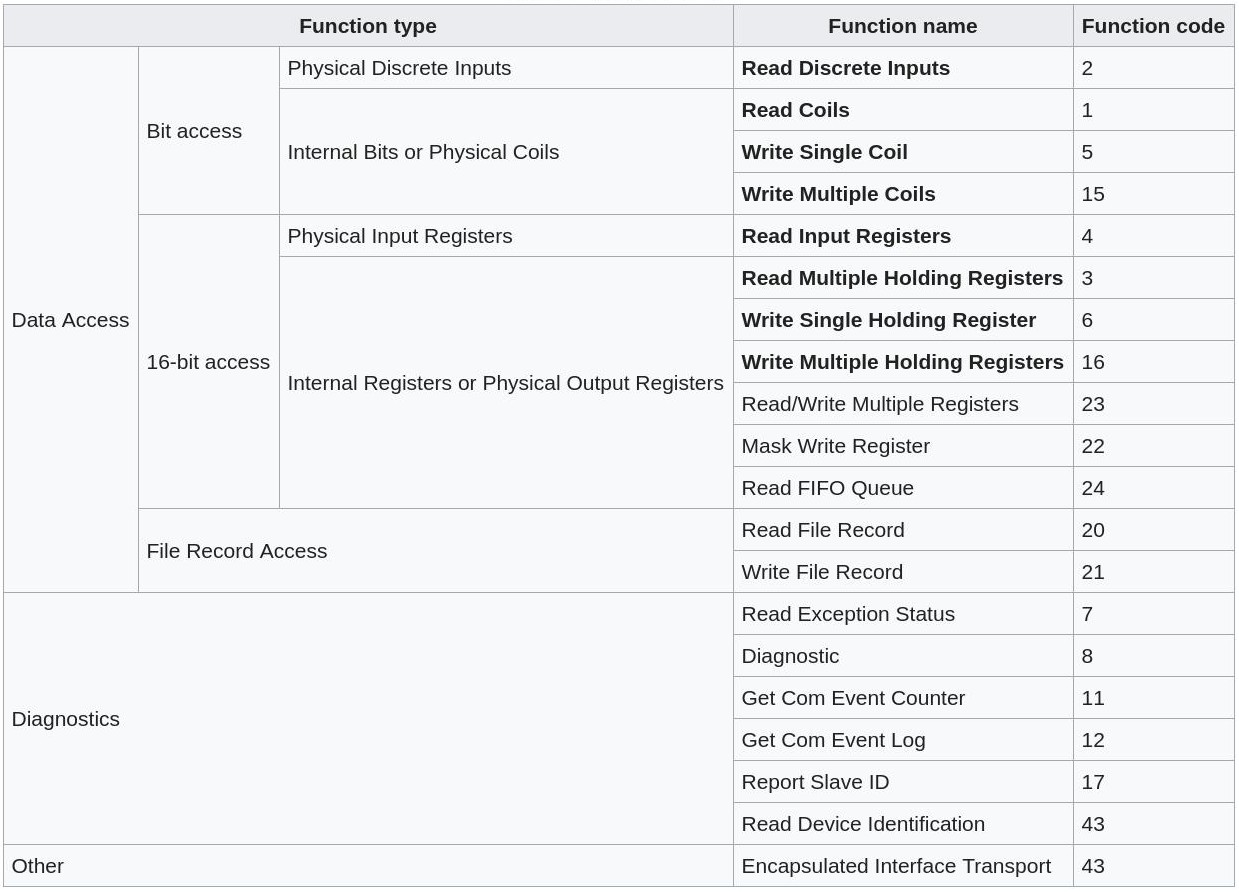
\includegraphics[width=0.9\linewidth]{modbusinstrukcje}
		\caption{Instrukcje protokołu
			\cite{image:modbus}}
		\label{fig:modbusinstrukcje}
	\end{figure}	
}

\frame{
	\frametitle{Modbus}
	\begin{figure}
		\centering
		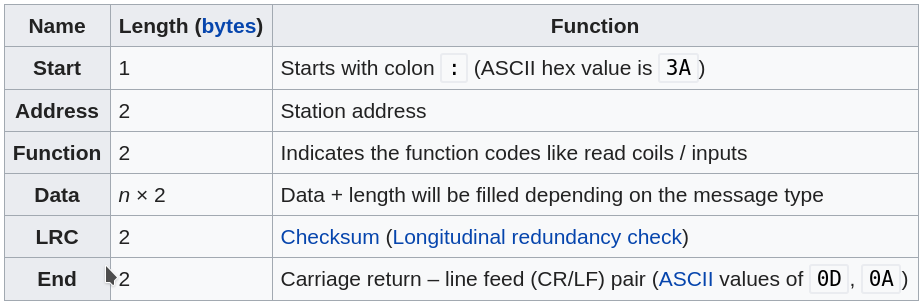
\includegraphics[width=0.9\linewidth]{modbusrtu}
		\caption{Instrukcje protokołu dla RS-485
			\cite{image:modbus}}
		\label{fig:modbusrtu}
	\end{figure}	
	\begin{figure}
		\centering
		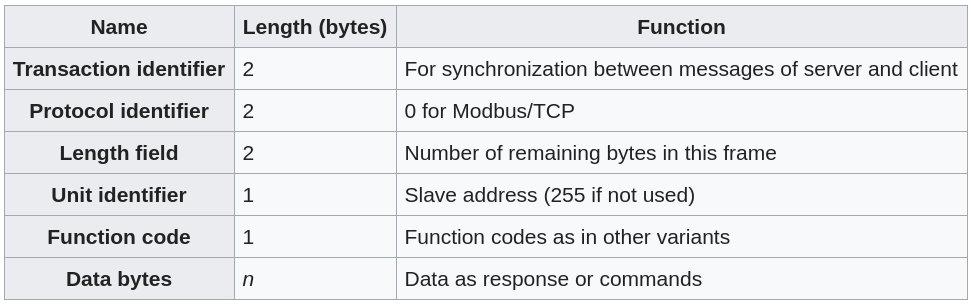
\includegraphics[width=0.9\linewidth]{modbusramka}
		\caption{Instrukcje protokołu dla TCP/IP
			\cite{image:modbus}}
		\label{fig:modbusramka}
	\end{figure}	
}



\frame{
	\frametitle{CAN}
	
}
\frame{
	\frametitle{CANOpen}
}

\frame{
	\frametitle{I$^2$C}
	\begin{itemize}
		\item Połączenie równoległe
		\item 5 Mbit/s
		\item $[2.3 - 5.5]$ V
		\item max. pojemność szyny: 400pF (kilka metrów)
		\item Pull-upy
		\item W praktyce najczęściej jeden master
		\item Wstrzymywanie zegara
	\end{itemize}
	\begin{itemize}
		\item \textbf{SDA}: Dane
		\item \textbf{SCL}: Zegar
	\end{itemize}
}


\frame{\frametitle{I$^2$C}
	\begin{figure}
		\centering
		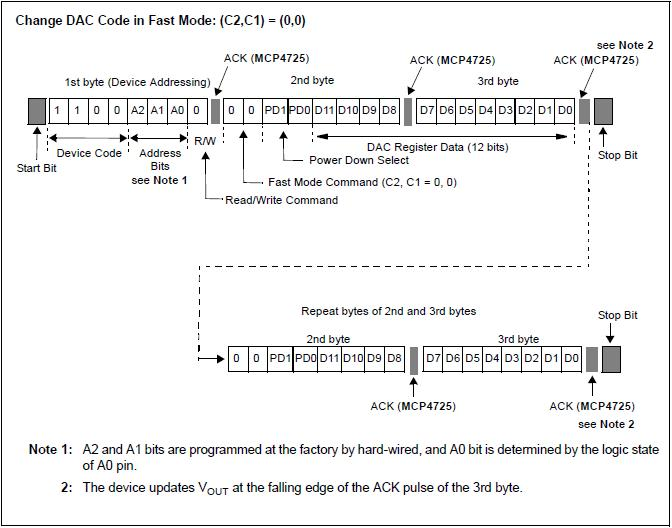
\includegraphics[width=0.9\linewidth]{i2c}
		\caption{Ramka szyny I2C
			\cite{image:i2c}}
		\label{fig:i2c}
	\end{figure}	
	}

\frame{
	\frametitle{USB}
	\begin{itemize}
		\item 5 m
		\item 127 urządzeń
	\end{itemize}
	\begin{itemize}
		\item v2.0 -> 480Mbit/s; 100 mA
		\item v3.1 Gen 2 -> 10Gbit/s; 900 mA 
		\item USB-C; 3 A
		\item Power Delivery USB; moc do 140 W
		\item OMTP/GSMA
	\end{itemize}
	
	\begin{itemize}
		\item Koncentratory
		\item Plug and Play
		\item Bezprzewodowy USB
	\end{itemize}
}
\frame{
	\frametitle{USB}	
	Pojedynczy host odpytuje wszystkie urządzenia cyklicznie. Urządzenia nie inicjują transmisji.\\
	Kanały:
	\begin{itemize}
		\item pipes
		\item logiczne
		\item 16 in, 16 out
		\item stream: jednokierunkowa, do przesyłu
		\item wiadomość: dwukierunkowa, do kontroli 
		\item huby
	\end{itemize}
	
	Podłączenie:
	\begin{itemize}
		\item Reset
		\item Enumeracja
		\item Przydzielenie kanałów
	\end{itemize}

}

\frame{
	\frametitle{USB}
	\begin{figure}
		\centering
		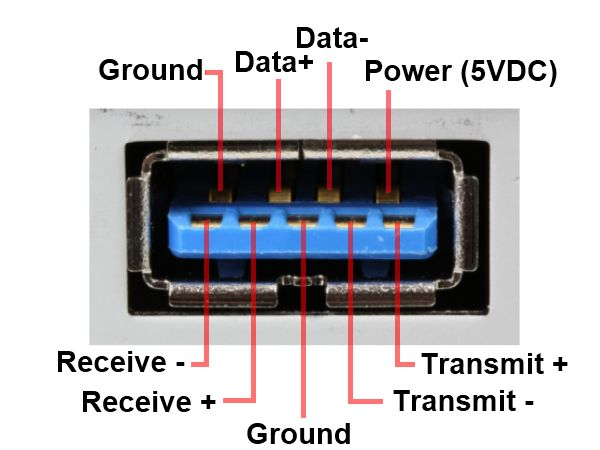
\includegraphics[width=0.9\linewidth]{usb3pinout}
		\caption{Złącza USB
			\cite{image:usbpinout}}
		\label{fig:usb3pinout}
	\end{figure}
}

\frame{
	\frametitle{USB}
	\begin{figure}
		\centering
		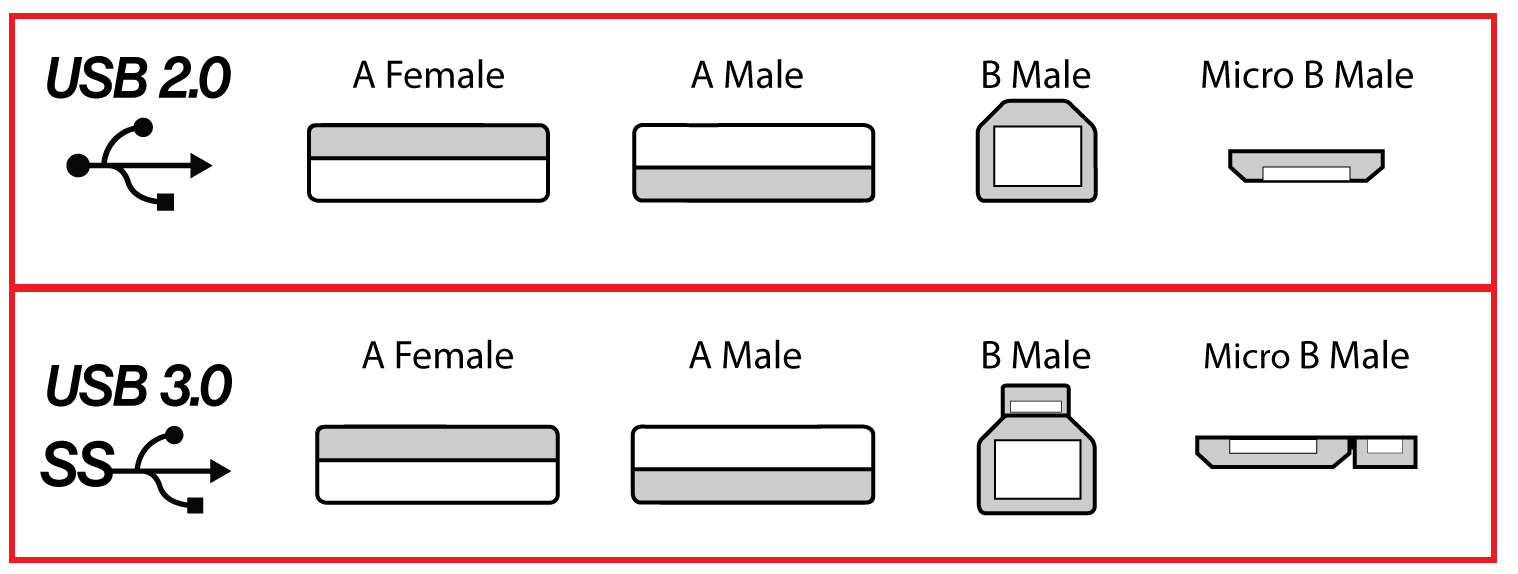
\includegraphics[width=0.9\linewidth]{usbconnectors}
		\caption{Złącza USB
			\cite{image:usbconnectors}}
		\label{fig:usbconnectors}
	\end{figure}
	\begin{figure}
		\centering
		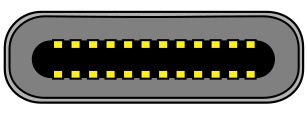
\includegraphics[width=0.3\linewidth]{usb3c}
		\caption{Złącza USB
			\cite{image:usbconnectors}}
		\label{fig:usb3c}
	\end{figure}
	}

\frame{
	\frametitle{Ethernet - kable miedziane}
	\begin{itemize}
		\item Złącze 8P8C
		\item Topologia gwiazdy
		\item Połaczenia proste pomiędzy switchami i komputerami
		\item Połączenia krosowane pomiędzy dwoma switchami lub dwoma komputerami
		\item Odległość transmisji wynosi 100 m
	\end{itemize}
}


\frame{\frametitle{WiFi}
	\begin{itemize}
		\item Half-duplex
		\item Nie wszystkie urządzenia się widzą
	\end{itemize}}
	\begin{itemize}
		\item 
	\end{itemize}


\frame{
	\frametitle{Ethercat}	
}

\frame{
	\frametitle{Gigavision}	
}


\section{Przykłady praktyczne}

\frame{
	\frametitle{Serwonapęd}	
}

\frame{
	\frametitle{Czujnik siły}
	
}

\frame{
	\frametitle{IRp-6}
}

\frame{
	\frametitle{Velma}	
}


\frame{
	\frametitle{Bibliografia}
	\bibliographystyle{plain}
	\bibliography{bibliography}
}

\section{Podsumowanie}
\frame{
	\frametitle{Literatura}
	\bibliography{bibliography}
}

\end{document}
